% !TEX encoding = UTF-8
% !TEX TS-program = pdflatex
% !TEX root = ../tesi.tex

%**************************************************************
\chapter{Progettazione e codifica}
\label{cap:progettazione}
In questo capitolo verrà tratta il secondo periodo del tirocinio: la progettazione e la codifica. Questa parte, avvenuta dopo l'Analisi dei Requisiti, è da ritenersi importante per progetto in quanto ha occupato gran parte del tempo lavorativo. Il primo passo è stato eseguire la progettata dell'architettura, in modo che i servizi necessari fossero correttamente configurati prima del loro effettivo utilizzo. Successivamente è stata eseguita la stesura del codice per la realizzazione della Skill. Nei paragrafi successivi seguiranno porzioni di codice significativo per la loro importanza e per il funzionamento di determinate funzionalità e/o servizi. Importante ricordare che il codice implementato e mostrato sarà in Node.js come quanto detto nel nel paragrafo \hyperref[nodejs]{1.4.1}. 
%**************************************************************
\section{Architettura}
Come riportato nel paragrafo \hyperref[serivizi-aws]{1.4.3}, il progetto si basa interamente sui servizi offerti dall'ecosistema Amazon. Di conseguenza è risultato facile ed immediato impostare i servizi dell'architettura in modo da rendere il tutto efficacie ed efficiente. In questo paragrafo si andrà a comprendere cosa offre ogni singolo servizio di AWS e come esso è stato impostato per il suo corretto funzionamento nella Skill.

\section{Configurazione servizi Amazon Web Service}
\subsection{AWS SES}
Amazon SES\footnote{AWS SES. URL: \href{https://aws.amazon.com/it/ses/}{https://aws.amazon.com/it/ses/}} (Simple Email Service) è un servizio di invio e-mail basato sul cloud messo a disposizione da Amazon per gli sviluppatori di applicazioni. Tale servizio è da considerarsi vantaggioso in quanto è affidabile e a costo ridotto, utile per qualunque tipo di azienda ed ideale per la realizzazione del progetto.
\newpage
\noindent Per utilizzare AWS SES è necessario impostare il servizio visitando la pagina\footnote{AWS SES. URL: \href{https://aws.amazon.com/it/ses/}{https://aws.amazon.com/it/ses/}} dedicata ed eseguire le istruzioni riportate:
\\[0.5cm]
\begin{minipage}{0.5\textwidth}
	\begin{figure}[H]
		
\includegraphics[width=6cm]{immagini/ses.png}
		\caption{\label{fig:icona_aws_ses}Icona AWS SES}
	\end{figure}
\end{minipage}
\begin{minipage}{0.5\textwidth}
	\begin{itemize}
		\item Eseguire l'accesso con le proprie credenziali di account AWS;
    	\item Una volta fatto l'accesso cliccare \texttt{Email Addresses} sul pannello a sinistra;
    	\item Cliccare \texttt{Verify a New Email Address};
    	\item Inserire l'indirizzo e-mail da verificare il quale verrà utilizzato per inviare le notifiche;
    	\item Confermare la verifica cliccando sul URL contenuto nella e-mail ricevuta.
	\end{itemize}
\end{minipage}
\\[0.5cm]
Il procedimento descritto sopra non fa altro che verificare l'indirizzo e-mail con il quale si andrà ad inviare messaggi di posta elettronica tramite la Skill. Amazon infatti permette l'uso di questo servizio solo se il mittente e il destinatario delle e-mail sono indirizzi verificati. Per completare la configurazione è necessario di verificare il dominio delle caselle mail di Crispy Bacon: 
\begin{itemize}
    \item Sempre all'interno di AWS SES cliccare su \texttt{Domains} sul pannello a sinistra;
    \item Cliccare in altro \texttt{Verify a New Domains};
    \item Inserire il dominio degli indirizzi e-mail destinatari delle mail, nel caso del progetto \textit{crispybacon.store};
    \item Infine cliccare su \texttt{Verify This Domain} per terminare il processo di verifica.
\end{itemize}
A questo punto è possibile mandare messaggi e notifiche tramite mail utilizzando l'indirizzo verificato prima.
\newpage
\subsection{AWS S3}
Amazon S3\footnote{AWS S3. URL: \href{https://aws.amazon.com/it/s3/}{https://aws.amazon.com/it/s3/}} (S3 = Simple Storage Service) è un servizio di storage di oggetti che offre scalabilità, disponibilità dati, sicurezza e prestazioni all'avanguardia. Queste caratteristiche offre alle industrie di qualsiasi dimensione la possibilità di archiviare e proteggere una qualsiasi quantità di dati per qualunque genere di uso: come ad esempio per siti Web, applicazioni mobile, backup e ripristino, archiviazione, applicazioni enterprise\footnote{Iintegrazione tra diversi tipi di sistemi informatici con l'utilizzo di software e soluzioni architetturali}, dispositivi IoT\footnote{Internet of Things: neologismo utilizzato per dare un nome agli oggetti reali connessi ad internet} e analisi di big data. Amazon S3 offre una gestione semplice di utilizzo grazie alla sua pagina web dedicata, all'interno di AWS Console, che  di organizzare i dati e di configurare controlli di accesso. S3 vanta di avere clienti di grande notorietà come Netflix, Airbnb, Finra e altri ancora. Nel caso del progetto S3 è stato utilizzato per organizzare e archiviare file multimediali, per lo più immagini, necessari per la composizione delle schermate APL mostrate a video sul display del dispositivo utilizzato. Per caricare tali file è necessario seguire le seguenti istruzioni riportate:
\\[0.5cm]
\begin{minipage}{0.4\textwidth}
	\begin{figure}[H]
		
\includegraphics[width=6cm]{immagini/amazon-s3.png}
		\caption{\label{fig:icona_aws_s3}Icona AWS S3}
	\end{figure}
\end{minipage}
\begin{minipage}{0.6\textwidth}
	\begin{itemize}
		\item Effettuare l'accesso con le proprie credenziali di account AWS;
    	\item Una volta entrati nella pagina di S3 cliccare su \texttt{Crea bucket}\footnote{Un contenitore di oggetti memorizzato al suo interno} sul pannello di opzioni riportato in alto;
    	\item Apparirà una nuova finestra dove sarà necessario inserire il nome del bucket, nel caso del progetto \textit{concierge-corccante}, e la regione del server che ospiterà i dati, in questo caso \textit{UE Irlanda}. Infine cliccare su \texttt{Successivo} fino al termine della schermata lasciando invariate le impostazioni proposte;
    	\item A questo punto il bucket (contenitore) è stato creato. Per entrare basterà ora cliccare sul suo nome nella lista dei bucket.
	\end{itemize}
\end{minipage}
\\[0.5cm]
Il passo finale di questa configurazione sarà caricare i file multimediali che le schermate APL necessitano. Quindi una volta entrati nel bucket creato in precedenza:
\begin{itemize}
    \item Cliccare sul \texttt{Carica} sul pannello di opzioni riportato in alto;
    \item Apparirà una nuova finestra dove aggiungere uno più file cliccando su \texttt{Aggiungi};
    \item Per procedere cliccare su \texttt{Successivo} e alla seconda schermata impostare le autorizzazioni pubbliche su \textit{Concedi l'accesso pubblico..};
    \item Continuare cliccando su \texttt{Successivo} fino al termine della schermata lasciando invariate le impostazioni proposte.
\end{itemize}
Ora i file sono archiviati e organizzati, pronti per essere utilizzati dalle schermate APL.

\subsection{AWS IAM}
\label{aws-iam}
Amazon IAM\footnote{AWS IAM. URL: \href{https://aws.amazon.com/it/iam/}{https://aws.amazon.com/it/iam/}} (Identity and Access Management) consente di gestire in sicurezza l'accesso ai servizi e alle risorse di AWS. Con questo servizio di management è possibile creare ed amministrare utenti e gruppi di utenti in modo da autorizzare o negare loro l'accesso alle risorse di AWS. Per ovvie ragioni, IAM svolge un ruolo importante nel progetto in quanto abilita e disabilità l'uso di tutti i servizi di Amazon usati dalla Skill. È pertanto necessario porre particolare attenzione ai passaggi di configurazione del gestore di sicurezza così da garantire il corretto funzionamento del prodotto finale:
\begin{minipage}{0.4\textwidth}
	\begin{figure}[H]
		
\includegraphics[width=5cm]{immagini/amazon-iam.png}
		\caption{\label{fig:icona_aws_iam}Icona AWS IAM}
	\end{figure}
\end{minipage}
\begin{minipage}{0.6\textwidth}
	\begin{itemize}
		\item Eseguire l'accesso con le proprie credenziali di account AWS;
    	\item Una volta entrati bisognerà recarsi su \texttt{Policy} presente nel pannello a sinistra e cliccare su \texttt{Crea policy};
    	\item Si verrà indirizzati in una nuova pagina dove sarà necessario andare nella sezione \texttt{JSON} ed incollare il codice sotto riportato utilizzato per il progetto;
    	\item Infine cliccare su \texttt{Verifica policy}.
	\end{itemize}
\end{minipage}
\lstinputlisting[caption=Esempio Policy IAM]{code/policy.json}
Ora è necessario associare le policy create con le roles:
\begin{itemize}
	\item Quindi andare sulla sezione \texttt{Ruoli} presente nel pannello a sinistra e cliccare su \texttt{Crea ruolo};
	\item Nella nuova pagina selezionare il servizio che utilizzerà il nuovo ruolo, quindi scegliere \textbf{Lambda} e cliccare su \texttt{Successivo};
	\item La pagina successiva mostra l'elenco di policy disponibili, quindi scegliere la policy creata precedentemente e continuare cliccando su \texttt{Successivo};
	\item Completare la procedura seguendo le istruzioni della pagina;
	\item Terminato tale processo sarà ora possibile associare la role creata con la Lambda, che verrà fatto al momento della creazione, per permettere alla funzione di utilizzare i servizi AWS necessari.
\end{itemize}
\begin{figure}[H] 
    \centering 
    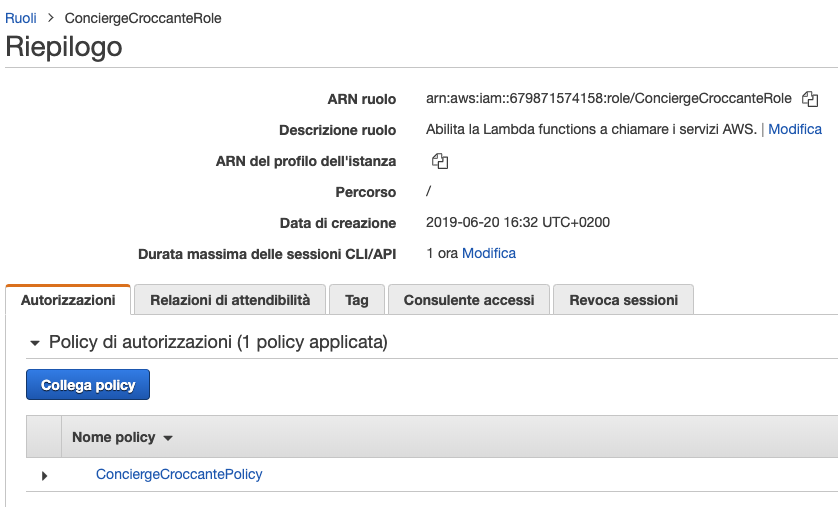
\includegraphics[width=1\columnwidth]{immagini/amazon-iam-role.png}
    \caption{\label{fig:esempio-amazon-iam-role}Esempio di Role creata}
\end{figure}

\newpage
\subsection{AWS CloudWatch}
Amazon CloudWatch\footnote{AWS CloudWatch. URL: \href{https://aws.amazon.com/it/cloudwatch/}{https://aws.amazon.com/it/cloudwatch/}} è un servizio di monitoraggio pensato per gli sviluppatori per fornire dati e analisi dal monitoraggio delle applicazioni, così da rispondere ai cambiamenti di prestazioni a livello di sistema, ottimizzare l'utilizzo delle risorse e ottenere una visualizzazione unificata dello stato di integrità operativa. CloudWatch raccoglie i dati di monitoraggio sotto forma di log, parametri ed eventi, unificando la loro visualizzazione, sulle applicazioni e i servizi eseguiti in AWS. Nel caso del progetto Concierce Croccante CloudWatch è stato utilizzato per rilevare comportamenti anomali della Skill, così da rilevare gli eventuali errori visualizzandone i log.
\begin{figure}[H] 
    \centering 
    
\includegraphics[width=0.8\columnwidth]{immagini/amazon-cloudwatch.png}
    \caption{\label{fig:icona_aws_cloudwatch}Icona AWS CloudWatch}
\end{figure}
\noindent Nel punto precedente, ovvero nel paragrafo \hyperref[aws-iam]{3.2.3}, è stato eseguito il procedimento necessario perché il servizio di CloudWatch venga abilitato. Pertanto non è necessario alcuna configurazione. Basterà recarsi al sito per poter utilizzare il servizio qualora si voglia visualizzare i dati sotto forma di log dopo o durante l'esecuzione di un servizio AWS, nel caso del progetto il servizio di AWS Lambda.

\subsection{AWS DynamoDB}
Amazon DynamoDB\footnote{AWS DynamoDB. URL: \href{https://aws.amazon.com/it/dynamodb/}{https://aws.amazon.com/it/dynamodb/}} è un servizio di database NoSQL (database non relazionale) proprietario e completamente gestito che supporta strutture di dati di tipo documento e di tipo chiave-valore. Caratteristiche di pregio sono database durevoli, multiregione e offrono sicurezza, backup, ripristino e cache in memoria per le applicazioni Internet. DynamoDB può gestire oltre 10 trilioni di richieste al giorno e supportando picchi di oltre 20 milioni di richieste al secondo. Nel progetto La Skill realizzata utilizza tale servizio per interrogare un database contenente la lista dei nomi del personale Crispy Bacon. 
\begin{figure}[H] 
    \centering 
    
\includegraphics[width=0.8\columnwidth]{immagini/amazon-dynamodb.png}
    \caption{\label{fig:icona_aws_dynamo}Icona AWS DynamoDB}
\end{figure}
\noindent È necessario quindi impostare tale servizio. Per farlo occorre recarsi nella pagina dedicata del db e una volta eseguito l'accesso con le proprie credenziali seguire le seguenti istruzioni:
\begin{itemize}
	\item Nel pannello a sinistra andare sulla sezione \texttt{Tabelle} e successivamente su \texttt{Crea Tabella}
	\item Nella nuova pagina sarà possibile settare le impostazioni della nuova tabella, quindi inserire un nome e due chiavi primarie, una di partizione e una di ordinamento, come mostra l'immagine seguente
	\begin{figure}[H] 
        \centering 
        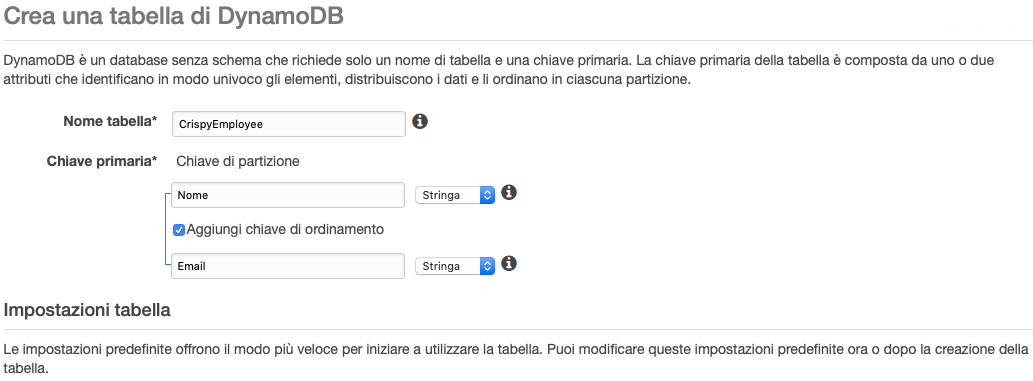
\includegraphics[width=1\columnwidth]{immagini/aws_dynamo.png}
	    \caption{\label{fig:esempio_aws_dynamo}Esempio creazione tabella AWS DynamoDB}
    \end{figure}
	
	\item Infine cliccare su \texttt{Crea}
\end{itemize}
Ora è possibile popolare il database inserendo i dati nell'apposito pannello di controllo di DynamoDB oppure fare delle interrogazioni da codice.

\newpage
\section{Creazione della Skill}
Una volta configurati correttamente tutti i servizi di AWS che Concierge Croccante andrà ad utilizzare si è proceduti con la realizzazione vera e propria della Skill. In questa parte infatti si andrà a mostrare e spiegare come questa sia stata realizzata basandosi sull'analisi della VUI fatta al punto \hyperref[vui]{2.5}. Il processo di realizzazione della Skill parte dalla console per sviluppatori di Alexa, a seguire la creazione della funzione Lambda dove verrà eseguito il programma, terminando infine con la stesura del codice mostrando parti di esso ritenute fondamentali. 
\subsection{Alexa Developer Console}
Per creare la Skill C.C. è necessario visitare ed entrare nella console di gestione ed accedere al servizio Alexa Skills Kit\footnote{Alexa Skill Kit. URL: \href{https://developer.amazon.com/it/alexa-skills-kit}{https://developer.amazon.com/it/alexa-skills-kit}}. Una volta fatto l’accesso con le proprie credenziali si è proceduto a creare il prodotto:
\begin{itemize}
	\item Cliccare su \texttt{Create Skill} per creare la Skill;\\
	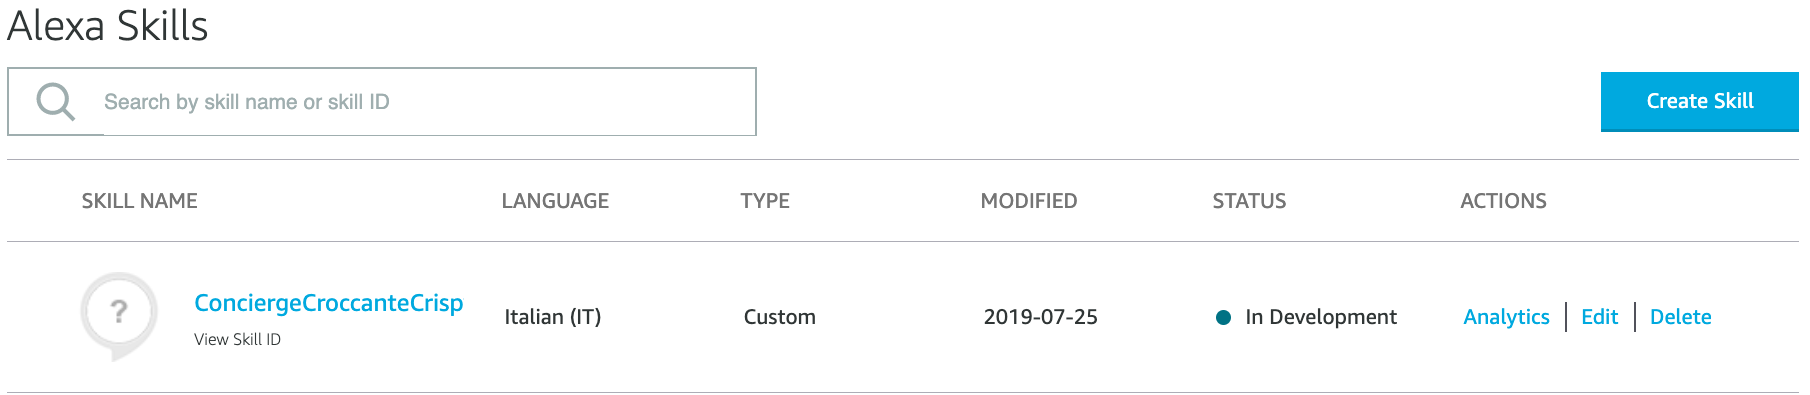
\includegraphics[width=12.5cm]{immagini/alexa-console-dev1.png}
	\item Nella pagina successiva, dare un nome alla propria Skill (facendo attenzione al fatto che quest'ultimo \textbf{non} sarà il nome di invocazione), scegliere la lingua, in questo caso \textit{Italian (IT)}, e scegliere \textit{Custom} come modello lasciando invariato il resto dei parametri. Successivamente cliccare nuovamente su \texttt{Create Skill};\\
	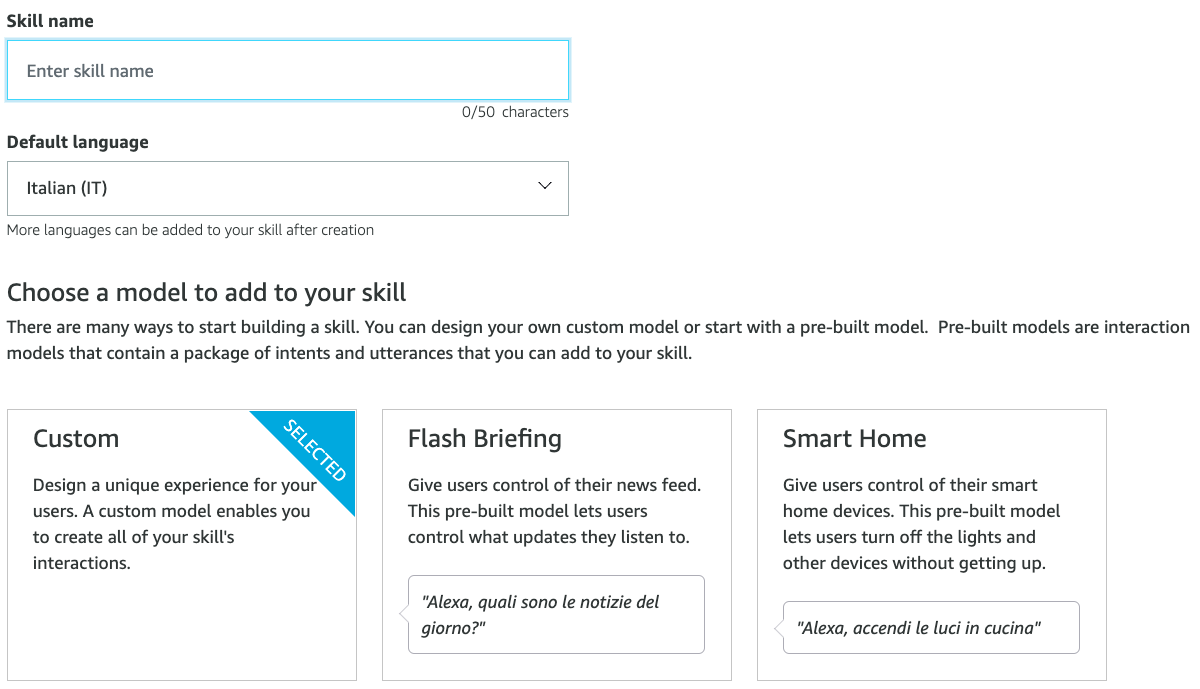
\includegraphics[width=13cm]{immagini/alexa-console-dev2.png}\\
	% 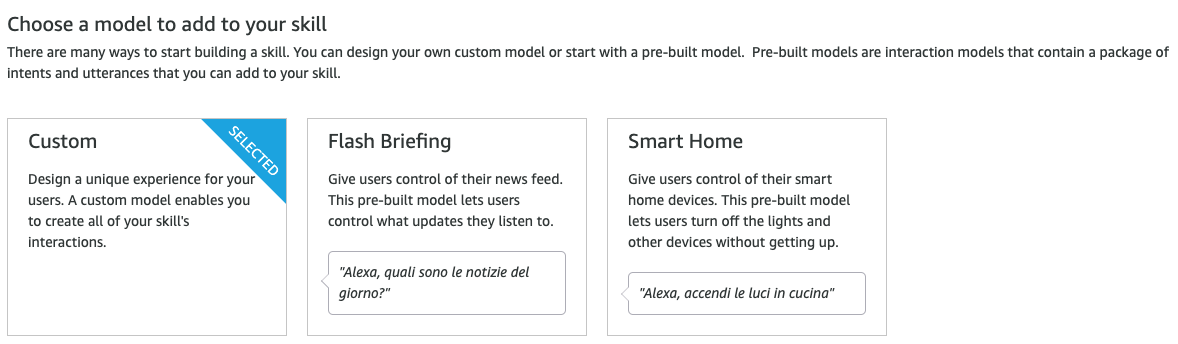
\includegraphics[width=12cm]{immagini/alexa-console-dev3.png}
	\newpage
	\item Si verrà reindirizzati nella pagina Alexa Developer Console dove sarà possibile customizzare la Skill. Nella sezione \texttt{Custom}, situata a sinistra, andare su \texttt{Invocation} per inserire il nome con cui si desidera invocare la Skill\\[0.5cm]
	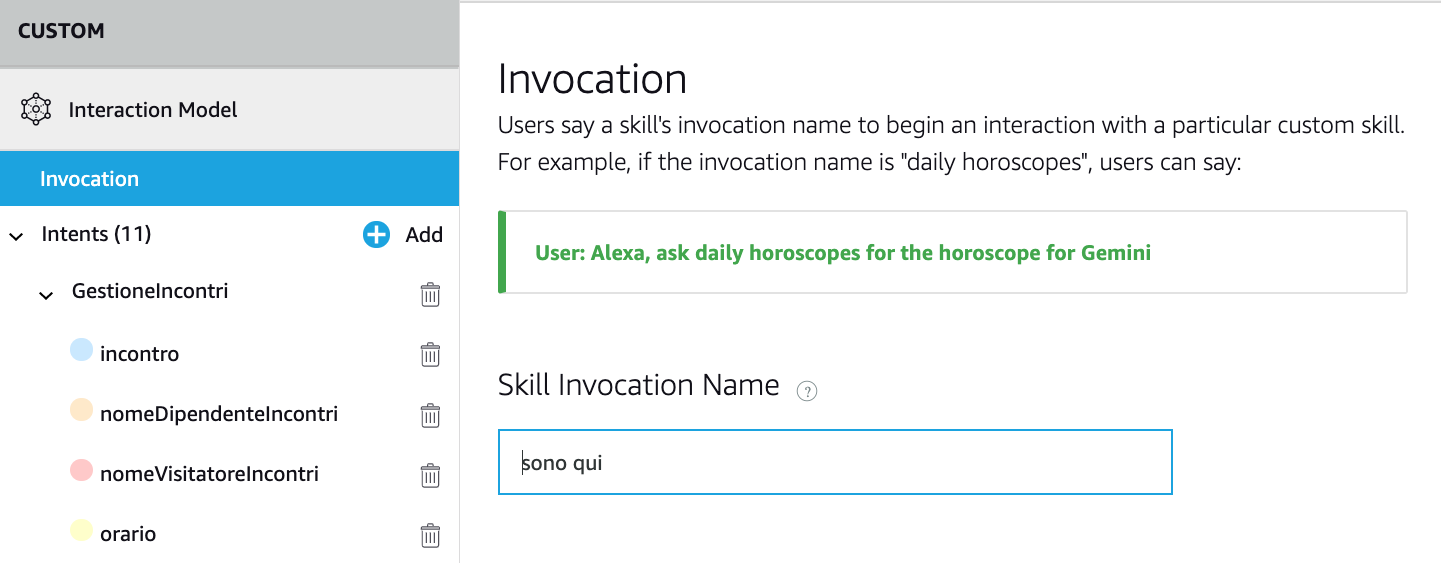
\includegraphics[width=12.5cm]{immagini/alexa-console-dev4.png}
	\item Successivamente è necessario creare gli intenti (\textit{intents}), che rappresentano un’azione che soddisfa una  richiesta del utente. Sempre nella sezione \texttt{Custom} - \texttt{JSON Editor} è possibile creari gli intenti caricando un file .json oppure scrivendoli sull'editor della pagina. A questo punto il comando di invocazione e gli intents sono stati impostati correttamente.\\[0.5cm]
	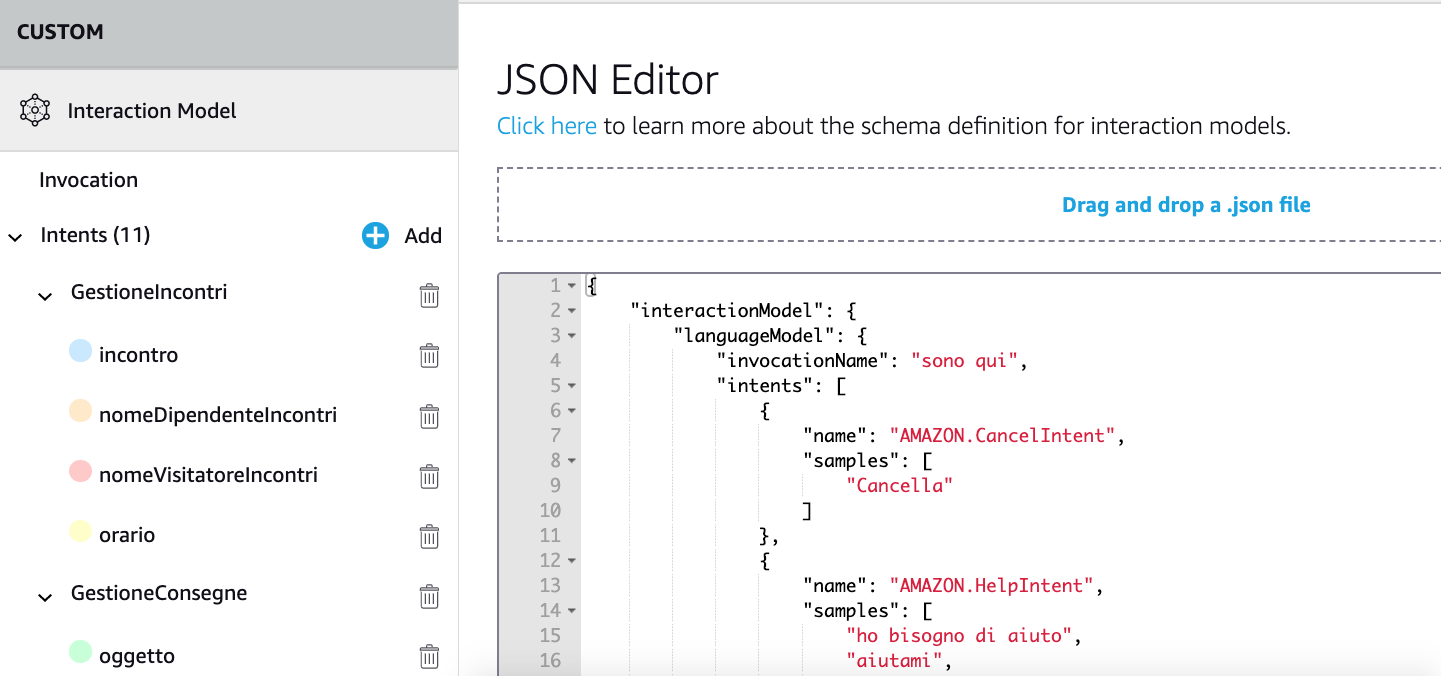
\includegraphics[width=12.5cm]{immagini/alexa-console-dev5.png}
\end{itemize}

\newpage
\noindent \subsubsection{Skill ID}
Il passo seguente è stato quello di salvare lo Skill ID, la chiave identificativa della Skill appena creata, che nei passi successi servirà per impostare l'endpoint: ovvero collegare la Skill alla Lambda dove risiederà il codice. Per fare ciò è stato sufficiente identificare e salvare l'ID inglobato nell'indirizzo URL della Skill appena creata, come mostra l'immagine seguente:
\begin{figure}[H]
	\centering
	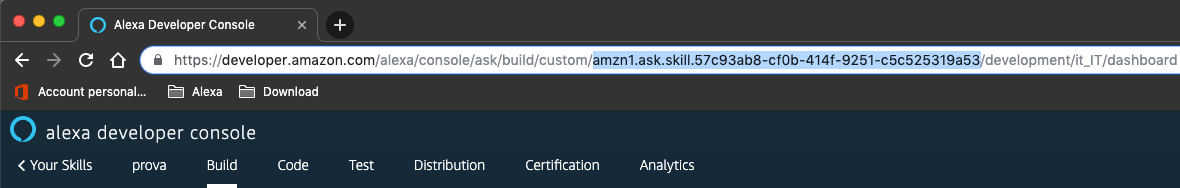
\includegraphics[width=13cm]{immagini/url_skill.png}
	\caption{Esempio Skill ID}
\end{figure}

\subsection{AWS Lambda}
Amazon Lambda\footnote{AWS Lamba. URL: \href{https://aws.amazon.com/it/lambda/}{https://aws.amazon.com/it/lambda/}} è un servizio della suite aws che consente di eseguire codice senza dover effettuare il provisioning\footnote{In telecomunicazioni è un servizi cloud a disposizione del utente che include hardware, software, cablaggio ed altro} e gestire server. Con Amazon Lambda è quindi possibile eseguire codice per qualsiasi tipo di applicazione o servizio back-end, senza alcuna amministrazione. Caricato il codice, Lambda attua tutte le azioni necessarie per eseguirlo e ricalibrare le risorse con massima disponibilità. È possibile anche configurare il codice in modo che venga attivato automaticamente da altri servizi AWS oppure che venga richiamato direttamente da qualsiasi applicazione Web o mobile.\\[0.5cm]
Una volta proceduti a creare la Skill la fese successiva è stata la realizzazione della funzione Lambda necessario per l'esecuzione del codice C.C.. Recandosi nell'omonima pagina, Amazon Lambda, sono stati eseguiti i passaggi di configurazione per creare la funzione ospitante il codice implementato o in fase di implementazione. Una volta fatto l'accesso con le proprie credenziali si è proceduto nel seguente modo:
\begin{minipage}{0.5\textwidth}
	\begin{figure}[H]
		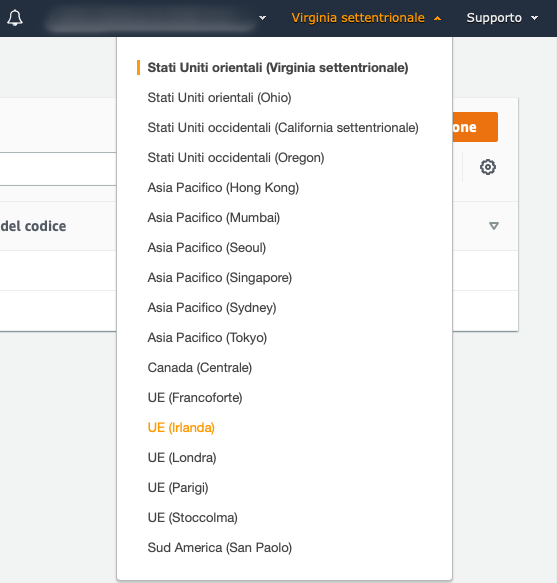
\includegraphics[width=6cm]{immagini/aws-lambda.png}
		\caption{\label{fig:aws_lambda_regione}Selezione regione AWS Lambda}
	\end{figure}
\end{minipage}
\begin{minipage}{0.5\textwidth}
	Prima di procedere è importate cambiare la regione di esecuzione della funzione Lambda. Quindi cliccare in alto a destra sulla regione (seconda voce) e scegliere \textit{UE (Irlanda)}, come mostrato in figura. Questo passaggio è necessario perché in base alla regione scelta, AWS - Lambda mette a disposizione più o meno servizi da integrare con la funzione. Tali informazioni possono essere reperite nell'apposita pagina\footnote{\href{https://amzn.to/30GkmTd}{https://amzn.to/30GkmTd}}. Di seguito viene fornito anche URL delle \href{https://amzn.to/2NCexm7}{Regioni ed endpoint AWS}\footnote{\href{https://amzn.to/2NCexm7}{https://amzn.to/2NCexm7}} dove sono riportate le informazioni degli endpoint di ogni servizio per ciascuna regione.
\end{minipage}
\begin{itemize}
	\item Cliccare in alto a destra su \texttt{Crea funzione} per creare la Lambda
	\item Nella pagina successiva, dare un nome alla funzione su cui verrà caricato il codice, nella sezione \texttt{runtime} scegliere \textit{Node.js 10.x} e infine nella sezione \texttt{Autorizzazioni} - \texttt{Ruolo di esecuzione} scegliere \textit{Utilizza ruolo esistente - ConciergeCroccanteRole} (ruole creato in precedenza durante la configurazione di AWS IAM al punto \hyperref[aws-iam]{3.2.3}). L'immagine seguente mostra la scelta corretta delle impostazioni base.\\[0.3cm]
	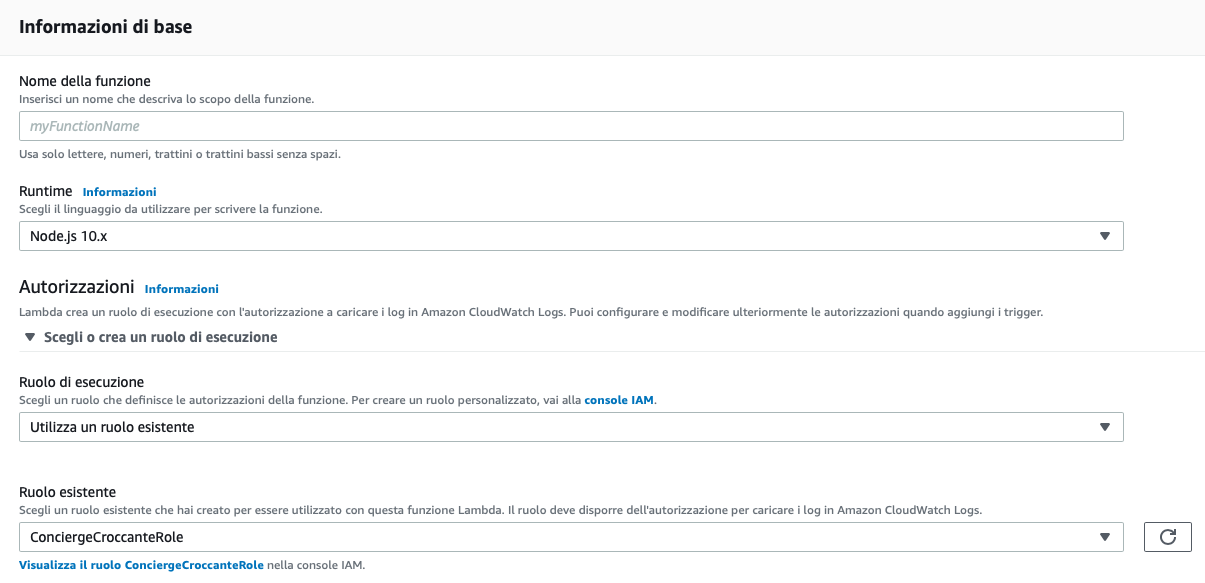
\includegraphics[width=13cm]{immagini/aws-lambda2}
	\item Successivamente cliccare nuovamente su \texttt{Crea funzione}
	\item Ora la funzione è stata impostata con le autorizzazioni sufficienti e necessarie per poter utilizzare i servizi che la Skill necessita. A destra cliccare su \texttt{Aggiungi trigger}, selezionare \texttt{Alexa Skill Kit}, inserire la Skill ID (salvata in precedenza) e cliccare su \texttt{Aggiungi} 
\end{itemize}
\subsubsection{Endpoint}
\label{endpoint}
Ora è possibile terminare il processo di configurazione della Skill eseguendo il collegamento tra Skill e Lambda. Ritornando nella console di AWS, sul servizio Lambda, è stato copiato l'indirizzo ARN della funzione, situato in alto a destra, come mostra nell'immagine seguente:
\begin{figure}[H]
	\centering
	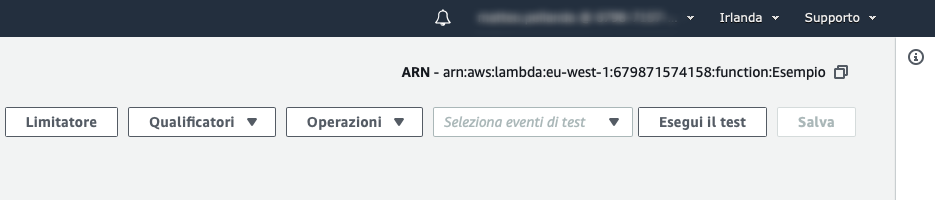
\includegraphics[width=13cm]{immagini/aws-lambda3.png}
	\caption{Esempio URL ARN Lambda}
\end{figure}
\noindent Successivamente, nella Skill in Alexa Developer Console, nella sezione \texttt{Custom} - \texttt{Endpoint}, incollare l'URL ARN della Lambda copiato in \texttt{Default Region}.
\begin{figure}[H]
	\centering
	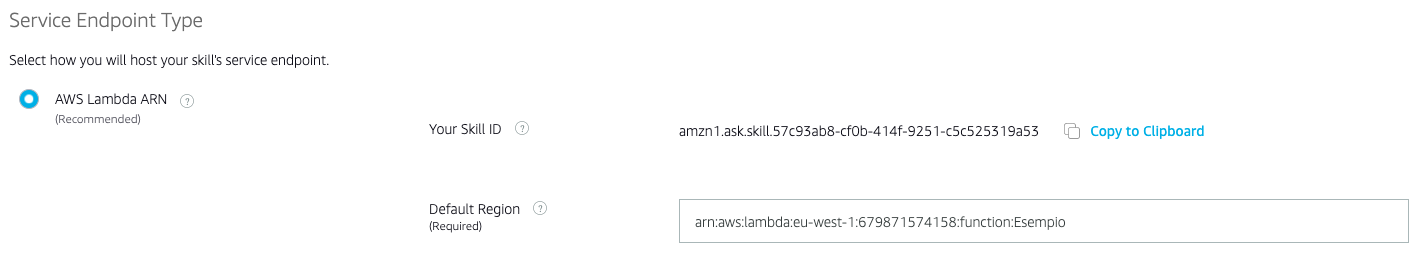
\includegraphics[width=13cm]{immagini/aws-lambda4.png}
	\caption{Esempio URL ARN Lambda}
\end{figure}
\noindent Infine cliccare su \texttt{Save Endpoint}. Ora la Skill l'endpoint impostato con l'esecuzione della funzione lambda creata.\\
Non rimane altro che caricare il codice del prodotto. Per farlo basterà recarsi nuovamente sulla console di AWS nel servizio Lambda, scegliere la propria funzione e su \texttt{Codice della funzione} scegliere \textit{Carica un file .zip} per caricare la cartella compressa del progetto.
\begin{figure}[H]
	\centering
	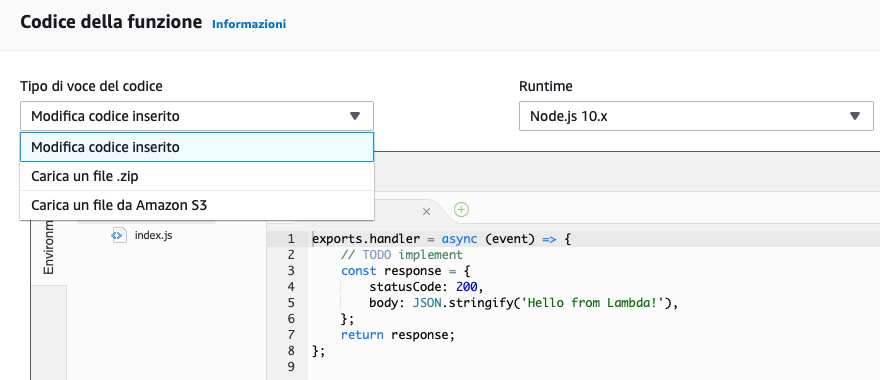
\includegraphics[width=13cm]{immagini/aws-lambda5.png}
	\caption{Codice funzione}
\end{figure}

\section{Organizzazione del codice}
Successiva alla parte di comprensione e configurazione dei servizi utilizzati in questo progetto, e alla creazione della Skill, è stato eseguito un micro-processo di organizzazione del codice prima della sua stesura. Questa pratica adottata è stata necessaria per avere uno schema e una gerarchia delle parti di codice che sono state sviluppate durante il periodo di tirocinio. Tale organizzazione ha permesso di sviluppare in maniera più ordinata e consapevole riducendo la probabilità di introdurre errori e rendendo il codice più manutenibile. Pertanto la cartella del progetto è stata così disposta:
\begin{itemize}
        \item \texttt{Skill}: cartella principale del progetto (main folder) contenente al suo interno altre cartelle e file organizzati secondo una determinata gerarchia
        \begin{itemize}
            \item[>] \texttt{apl-data}: cartella contenente i dati delle schermate APL
            \item[>] \texttt{apl-template}: cartella contenente i template lo stile delle schermate APL
            \item[>] \texttt{hendelrs}: cartella contenente i file .js di ogni handlers (gestori) creati nella Skill
            \item[>] \texttt{i18n}: cartella contente file .js con le traduzioni della lingua 
            \item[>] \texttt{node\_modules}: cartella contenente tutti i pacchetti installati con il gestore npm
            \item[>] \texttt{task}: cartella contente file .js da eseguire a riga di comando per l'esecuzione di funzionalità primitive 
            \item[>] \texttt{utils}: cartella contente file .js con classi di utilità, come lettura del db, invio di e-mail, ecc..
            \item[-] \texttt{credentials.json}: file contenente delle credenziali per accedere al servizio di Google Calendar
            \item[-] \texttt{googleAuthTokenCredential.json}: file contenente delle credenziali per accedere al servizio di Google Calendar
            \item[-] \texttt{index.js}: file principale dove inizia l'esecuzione della Skill. La Lambda difatti partirà con la lettura di questo file
            \item[-] \texttt{intent.json}: file .json contenente tutti gli intent creati per la Skill
            \item[-] \texttt{package.-lock.json}: file di configurazione automaticamente creato dal gestore di pacchetti npm
            \item[-] \texttt{package.json}: file di configurazione automaticamente creato dal gestore di pacchetti npm
            \item[-] \texttt{policy.json}: file .json contente le regole di policy create al punto \hyperref[aws-iam]{3.2.3}
        \end{itemize}
    \end{itemize}
\begin{figure}[H]
	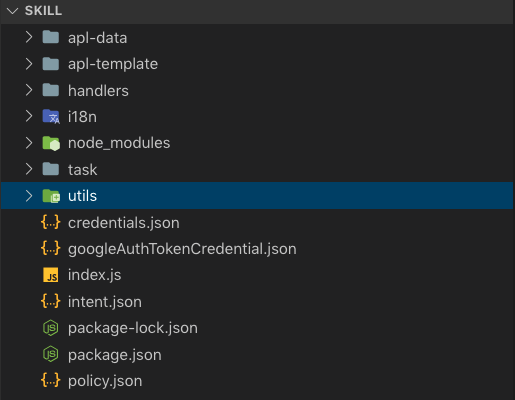
\includegraphics[width=13cm]{immagini/skill-folder.png}
	\caption{\label{fig:gerarchia_cartella_cc}Gerarchia cartella progetto C.C.}
\end{figure}

\subsection{Handlers}
Come descritto prima la cartella del progetto C.C. è stata disposta per una gestione ordinata del codice. Una delle sotto-cartelle contenute al suo interno è dedicata per la gestione degli handelrs. Nel codice della Skill gli handerls sono delle funzioni che hanno lo scopo di gestire gli intenti che vengono scatenati all'invocazione di un comando da parte dell'utente. Gli handlers sono stati così realizzati:
\begin{itemize}
    \item \texttt{index.js}: che contiene ed ingloba l'export di tutte le classi dei handlers contenuti in questa cartella
    
    \item \texttt{gestioneConsegne\_Complete.js}: questo handler ha il compito di catturare l'evento nel caso in cui l'utente intenda consegnare un pacco (o lettera) sapendo già il nome del destinatario e, o l'oggetto consegnato o la professione dell'utente che sta conversando
    \item \texttt{gestioneConsegne\_NomeDipendete.js}: questo handler ha il compito di catturare l'evento nel caso in cui l'utente intenda consegnare un pacco (o lettera) senza sapere già il nome del destinatario. Questo gestore ha il compito di richiedere tale dato domandandolo all'utente che sta conversando con la Skill
    \item \texttt{gestioneIncontri\_Complete.js}: questo handler ha il compito di catturare l'evento nel caso in cui l'utente visitatore abbia un appuntamento e i dati necessari sono stati tutti raccolti
    \item \texttt{gestioneIncontri\_NomeDipendente\_NomeVisitatore.js}: questo handelr ha il compito di catturare l'evento nel caso in cui l'utente visitatore abbia un appuntamento e, il nome del dipendetene cercato e del cliente appena entrato, sono stati raccolti. Il gestore eseguirà dei controlli per verificare l'attendibilità dei dati per poi proseguire con il dialogo oppure chiedendone di nuovi dati
    \item \texttt{gestioneIncontri\_NomeDipendente.js}: questo handler ha il compito di catturare l'evento nel caso in cui l'utente abbia un appuntamento e la Skill richiede il nome del dipendente cercato
    \item \texttt{gestioneIncontri\_Orari.js}: questo handler ha il compito di catturare l'evento nel caso in cui l'utente abbia un appuntamento e la Skill richiede l'orario per verificare l'evento nel calendario
    \item \texttt{vorreiIncontri\_Complete.js}: questo handler ha il compito di catturare l'evento nel caso in cui l'utente visitatore desideri incontrare un dipendente e sono stati raccolti tutti i dati necessari 
    \item \texttt{vorreiIncontri\_CompleteWithOrario.js}: questo handler ha il compito di catturare l'evento nel caso in cui l'utente visitatore desideri incontrare un dipendente e richiede l'orario di appuntamento per verificare l'esistenza dell'evento nel calendario 
    \item \texttt{vorreiIncontri\_NomeDipendente\_NomeVisitatore.js}: questo handler ha il compito di catturare l'evento nel caso in cui l'utente visitatore desideri incontrare un dipendente e, il nome del dipendetene cercato e del cliente appena entrato, sono stati raccolti. Il gestore eseguirà dei controlli per verificare l'attendibilità dei dati per poi proseguire con il dialogo oppure chiedendone di nuovi dati
    \item \texttt{vorreiIncontri\_NomeDipendente.js}: questo handler ha il compito di catturare l'evento nel caso in cui l'utente visitatore desideri incontrare un dipendente e la Skill richiede il nome di quest'ultimo
    \item \texttt{vorreiIncontri\_SiNo.js}: questo handler ha il compito di catturare l'evento nel caso in cui l'utente visitatore abbia un appuntamento e la Skill ne richiede l'orario per verificare l'evento nel calendario
    \item \texttt{touchWrapperUserEvent.js}: questo handler ha il compito di catturare gli eventi scatenati dal tocco sul display 
\end{itemize}
\begin{figure}[H]
	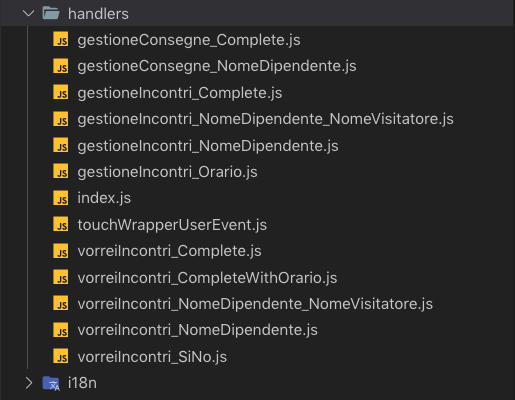
\includegraphics[width=13cm]{immagini/skill-folder2.png}
	\caption{\label{fig:gerarchia_cartella_cc2}Gerarchia cartella progetto C.C. - Handlers}
\end{figure}
\subsection{Utils}
\label{utils}
Lo stesso criterio usato per gli handlers è stato adotta anche per le classi Javascript che contengono il codice delle funzionalità della Skill. La cartella \textit{utils} contiene appunto quei metodi che permetto ad esempio la lettura del databse, l'invio di e-mail, l'invio di notifiche e la lettura del calendario. Le utilità sono state così realizzate:
\begin{itemize}
    \item \texttt{databaseUtils.js}: questa classe mette a disposizione i metodi per interrogare il database e sono presenti le seguenti funzioni:
    \begin{itemize}
        \item[>] \texttt{getInstance()}
        \item[>] \texttt{runQuery(params: var)}
        \item[>] \texttt{runScan(params: var)}
        \item[>] \texttt{runPut(params: var)}
        \item[>] \texttt{checkEmployee(nome\_dipendente: var)}
    \end{itemize}
    \item \texttt{emailUtils.js}: questa classe mette a disposizione i metodi per l'invio di messaggi e-mail ed è presente la seguente funzione:
    \begin{itemize}
        \item[>] \texttt{sendMail(from: var, to: var, message: var, oggetto: var)}
    \end{itemize}
    \item \texttt{gcalendarUtils.js}: questa classe mette a disposizione i metodi per la lettura e verifica di eventi nel calendario e sono presenti le seguenti funzioni:
    \begin{itemize}
        \item[>] \texttt{listEvents(idCalendar: var)}
        \item[>] \texttt{checkEvent(events: var, email\_dipendente: var, nome\_visitatore: var, orarioEvento: var)}
        \item[>] \texttt{generateOAuth2Client()}
    \end{itemize}
    \item \texttt{gchatUtils.js}: questa classe mette a disposizione i metodi per l'invio di notifiche su Google Chat, funzionalità in fase di sviluppo fatta nell'ultimo periodo di tirocinio, e sono presenti le seguenti funzioni:
    \begin{itemize}
        \item[>] \texttt{sendNotify(type: var, message: var)}
        \item[>] \texttt{checkThread(type: var)}
        \item[>] \texttt{putThread(thread: var, thread\_type: var)}
    \end{itemize}
    \item \texttt{prepareQuery.js}: questa classe mette a disposizioni i metodi per ricevere le query di interrogazione che si desidera e sono presenti le seguenti funzioni:
    \begin{itemize}
        \item[>] \texttt{scanEmployee()}
        \item[>] \texttt{queryEmployee(nomeDipendente: var)}
        \item[>] \texttt{putThread()}
        \item[>] \texttt{updateThread(old\_thread: var, new\_thread: var)}
    \end{itemize}
    \item \texttt{slacknotifyUtils.js}: questa classe mette a disposizione i metodi per l'invio di notifiche su Slack e al suo interno sono presenti le seguenti funzioni:
    \begin{itemize}
        \item[>] \texttt{sendNotify(channel: var, message: var)}
        \item[>] \texttt{sendDirectlyNotify(member: var, MESSAGE: var)}
        \item[>] \texttt{addTag(toTag: var)}
        \item[>] \texttt{listMembersApl(intent: var)}
        \item[>] \texttt{getIdMember(toTag: var)}
        \item[>] \texttt{membersList()}
    \end{itemize}
    \item \texttt{abracadabraUtils.js}: questo metodo contiene un easter egg\footnote{Un easter egg in informatica è un contenuto di natura bizzarra e innocuo che gli sviluppatori nascondono all'interno del prodotto}
\end{itemize}
\begin{figure}[H]
	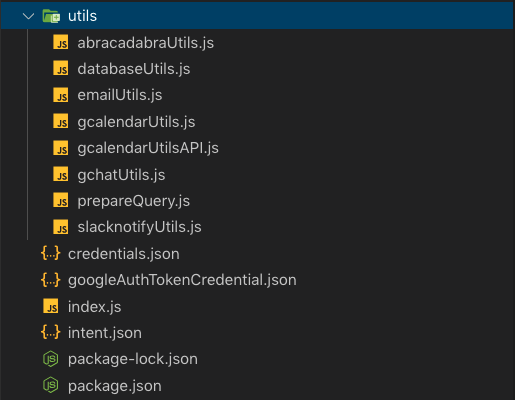
\includegraphics[width=13cm]{immagini/skill-folder3.png}
	\caption{\label{fig:gerarchia_cartella_cc3}Gerarchia cartella progetto C.C. - Utils}
\end{figure}

\section{Pacchetti}
Particolare attenzione va fatta sulla gestione dei pacchetti e quali di essi sono stati installati nel progetto Concierge Croccante. A tale necessità è stato utilizzato il gestore di pacchetti npm, menzionato in precedente al punto \hyperref[npm]{1.5.4}, che ha consentito di installare in maniera sicura e immediata i pacchetti necessari. Installando tali pacchetti il gestore ha suddiviso il codice all'interno di una directory chiamata \texttt{node\_modules} creando inoltre un file di configurazione delle installazioni fatte.
\begin{figure}[H]
	
\includegraphics[width=12cm]{immagini/logo-npm.png}
	\caption{\label{fig:logo_npm}Logo NPM}
\end{figure}
\noindent In questa fase di progetto si è provveduto ad installare npm e tutti i pacchetti necessari alla Skill Concierge Croccante nel seguente modo:
\begin{itemize}
    \item Dalla documentazione di npm\footnote{Doc npm. URL: \href{https://docs.npmjs.com/downloading-and-installing-node-js-and-npm}{https://docs.npmjs.com/downloading-and-installing-node-js-and-npm}} viene riportato il seguente comando da eseguire su terminale:
    \begin{lstlisting}[language=bash]
		$ [sudo] npm install npm -g
	\end{lstlisting}
	Il comando installerà l'ultima versione del gestore pacchetti. Se si desidera verificare e visualizzare l'ultima versione di npm è necessario eseguire il comando: 
	\begin{lstlisting}[language=bash]
		$ npm -v
	\end{lstlisting}
	\item I pacchetti installati nel progetto sono stati i seguenti:
	\begin{itemize}
	    \item[>] \texttt{ask-sdk} e \texttt{ask-sdk-core} di AWS che semplifica la creazione di Skill, permettendo di utilizzare le funzionalità base di Alexa in maniera rapida:
	    \begin{lstlisting}[language=bash]
		    $ npm install --save ask-sdk
		    $ npm install --save ask-sdk-core
	    \end{lstlisting}
	    \item[>] \texttt{request} per semplificare ed effettuare chiamate http, supporta HTTPS i re-indirizzamenti:
	    \begin{lstlisting}[language=bash]
		    $ npm install request
	    \end{lstlisting}
	    \item[>] \texttt{googleapis} è una libreria client per l'utilizzo delle API di Google, rendendo più semplice ed immediate le chiamate ai servizi come Calendar:
	    \begin{lstlisting}[language=bash]
		    $ npm install googleapis
	    \end{lstlisting}
	    \item[>] \texttt{slack-notify} è una libreria che rende flessibile l'utilizzo dell'API Webhooks\footnote{Incoming Webhooks. URL: \href{https://api.slack.com/incoming-webhooks}{https://api.slack.com/incoming-webhooks}} di Slack, semplificando l'invio di notifiche a Slack dalla Skill:
	    \begin{lstlisting}[language=bash]
		    $ npm install slack-notify
	    \end{lstlisting}
	    \item[>] \texttt{i18next} e \texttt{i18next-sprintf-postprocessor} sono dei framework di internazionalizzazione popolari ambienti javascript:
	    \begin{lstlisting}[language=bash]
		    $ npm install i18next
		    $ npm install i18next-sprintf-postprocessor
	    \end{lstlisting}
	\end{itemize}
\end{itemize}

\newpage
\section{Calendario}
Per la soddisfazione del requisito RO17 analizzato al punto \hyperref[requisti-richiesti]{2.3}, ovvero la lettura e verifica degli appuntamenti in calendario, è stato richiesto l'uso di Google Calendar, giù utilizzato dall'azienda Crispy Bacon per le sue note funzionalità. 
\subsection{Google Calendar}
Per l’integrazione col servizio di Google Calendar sono a disposizione delle API documentate reperibili al indirizzo \href{https://developers.google.com/calendar/}{developers.google.com/calendar/}. Dalla guida emergono i seguenti requisti necessari:\\
\begin{minipage}{0.5\textwidth}
	\begin{figure}[H]
		
\includegraphics[width=5cm]{immagini/google_calendar.png}
		\caption{\label{fig:icona_google_calendar}Icona Google Calendar}
	\end{figure}
\end{minipage}
\begin{minipage}{0.5\textwidth}
	\begin{itemize}
		\item Node.js
    	\item googleapis package
    	\item Account Google funzionante e verificato
    	\item Autorizzazione OAuth\footnote{OAuth: protocollo di rete open e standard, progettato per lavorare con il protocollo HTTP.}
	\end{itemize}
\end{minipage}
\\[0.5cm]
Nei punti successivi verranno analizzati aspetti importanti, con esempi di codice, riguardante l'integrazione con il calendario in questione e l’uso delle sue API.
\subsubsection{OAuth2}
Per consentire la lettura ed ottenere la lista di eventi presenti nel calendario è stato necessario eseguire un'autenticazione tramite il protocollo OAuth 2.0\footnote{OAuth 2.0. URL: \href{https://oauth.net/2/}{https://oauth.net/2/}}. Quest'ultimo è un protocollo di rete open che consente l'emissione di un token di accesso da parte di un server autorizzato ad un client di terze parti, nel nostro caso il servizio di Google Calendar, previa approvazione dell'utente proprietario della risorsa cui si intende accedere. Per poter ottenere ciò sono stati svolti i seguenti passi:
\begin{itemize}
    \item Visitando la pagina Google Calendar API\footnote{G. Calendar API. URL: \href{https://developers.google.com/calendar/quickstart/nodejs}{https://developers.google.com/calendar/quickstart/nodejs}} è stato abilitato l'utilizzo delle API per il calendario. Nella pagina infatti è presente il primo step da seguire dal titolo ”\textit{Turn on the Google Calendar API}” dove presente il bottone adibito all'abilitazione:\\
    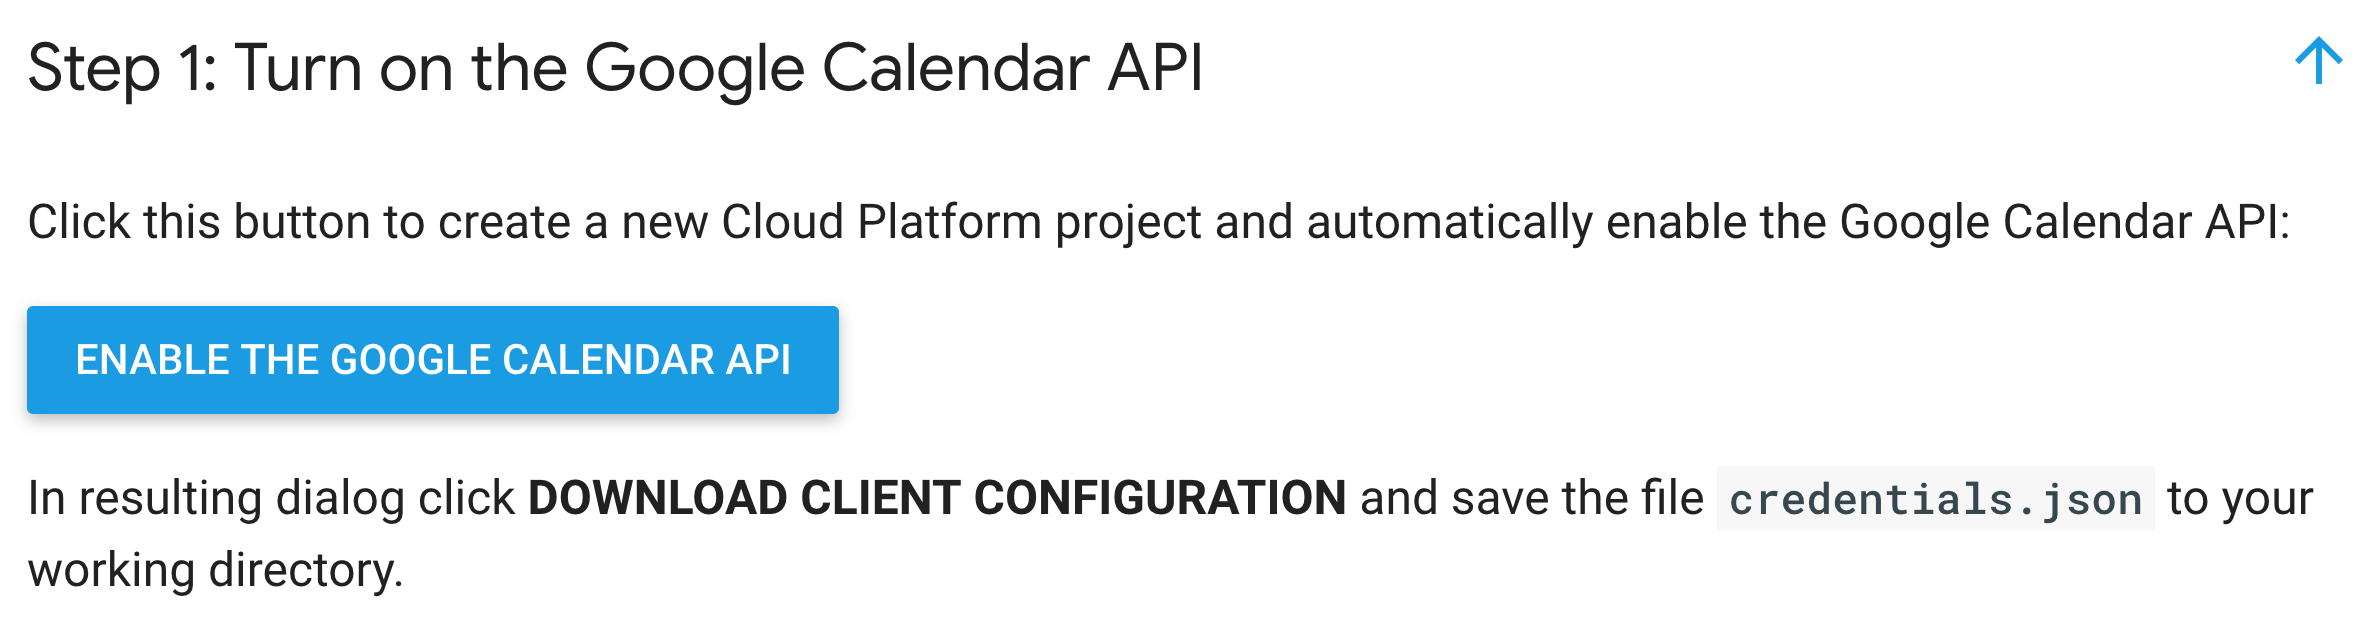
\includegraphics[width=12cm]{immagini/google_calendar_api.png}\\[2cm]
    Nella sezione corrente, una volta cliccato il bottone \texttt{ENABLE THE GOOGLE CALENDAR API} ed eseguito l’accesso con l’account Google il quale si desidera leggere gli eventi in calendario, è stato salvato il file credentials.json ottenuto dall'accesso e fornito nella cartella di progetto.
    \item Sempre nella stessa pagina è stato copiato ed eseguito l'esempio di set up riportato per ottenere l’OAuth necessario a visualizzare gli eventi nel calendario. Di seguito si riporta tale esempio di codice, importante appunto per ricevere le autorizzazioni necessarie:
	\lstinputlisting[caption=Esempio Set up Google Calendar]{code/generateGoogleAuthToken.js}
	\item Per eseguire tale esempio di codice è stato sufficiente aprire il terminale sulla cartella di progetto dove risiede il file di set up e lanciare lo script con il seguente comando:
	\begin{lstlisting}[language=bash]
		$ node [filename]
	\end{lstlisting}
	Nel caso in cui fossa la prima volta che eseguito tale esempio è necessario autorizzare l'accesso:
	\begin{enumerate}
		\item Aprire l'URL restituito dal terminale col proprio web browser
		\item Fare il login in se non si è già loggati
		\item Cliccare il bottone \texttt{Accept}
		\item Copiare il codice ricevuto, incollarlo nella terminale e premere \texttt{Enter}
	\end{enumerate}
\end{itemize}
\subsubsection{Lettura eventi}
All'interno del progetto Concierge Croccante la fase di lettura del calendario è stata semplificata realizzando una classe contenente al suo interno metodi appositi. Di tali metodi, già menzionati al punto \hyperref[utils]{3.4.2}, ne viene riportato il codice e analizzato il loro funzionamento:
\lstinputlisting[caption=Metodi listEvent e generateOAuth2Client]{code/gcalendarUtils1.js}
Per ottenere la lista di eventi non servirà altro che richiamare \texttt{listEvents(idCalendar)}. La funzione ritornerà un oggetto contenente tutti gli eventi, con le loro informazioni, della giornata odierna fino ad un massimo di 15 risultato. Attenzione: i file citati credentials.json e googleAuthTokenCredential.json non sono altro che le credenziali recuperate nei punti precedenti per accedere con il token OAuth.
\\[0.5cm]
Altro metodo presente e largamente utilizzato è \texttt{checkEvent(events, email\_dipendente, nome\_visitatore, orarioEvento)}:
\lstinputlisting[caption=Metodo checkEvent]{code/gcalendarUtils2.js}
Questo metodo pone come precondizione il fatto di ricevere in ingresso l'elenco di eventi ed i valori: nome visitatore, nome persona cercata ed orario; non vuoti. Il risultato sarà un valore \textit{boolean false} nel caso \textbf{non} sia presente alcun evento nel calendario, un valore numerico \textit{1} nel caso sia stato trovato un evento per la persona e l'orario indicato, oppure \textit{0} se esiste un evento ma l'orario indicato non coincide con quello effettivo.

\newpage
\section{Invio notifiche}
Altra specifica per la soddisfazione dei requisiti RO18 e RO19 analizzati al punto \hyperref[requisti-richiesti]{2.3}, è l'invio di notifiche. Per ovviare a ciò sono state realizzate le funzionalità per l'invio di messaggi istantanei via Slack e e-mail via AWS SES visto il già utilizzo di questi servizi da parte di Crispy Bacon.
\subsection{Slack}
Per l’integrazione col servizio di Slack sono a disposizione delle API documentate reperibili al indirizzo \href{https://api.slack.com/}{api.slack.com/}. Dalla guida emergono i seguenti requisti necessari:
\\
\begin{minipage}{0.5\textwidth}
	\begin{figure}[H]
		
\includegraphics[width=6cm]{immagini/slack.png}
		\caption{\label{fig:icona_slack}Icona servizio - Slack}
	\end{figure}
\end{minipage}
\begin{minipage}{0.5\textwidth}
	\begin{itemize}
		\item Node.js
		\item slack-notify package
		\item Account Slack
		\item Incoming Webhook
	\end{itemize}
\end{minipage}
\\[0.4cm]
Nei punti successivi verranno analizzati aspetti importanti, con esempi di codice, riguardante l'invio di notifiche con Slack e l’uso delle sue API.
\subsubsection{Incoming Webhooks}
Per consentire l'invio di messaggi di notifica via chat viene scelto di utilizzare un bot con Incoming Webhook\footnote{\href{https://it.wikipedia.org/wiki/Webhook}{https://it.wikipedia.org/wiki/Webhook}}. Quest'ultimo è un mezzo con il quale si semplifica l'invio di messaggi da un'applicazione a Slack. La creazione di un Incoming Webhook fornisce un URL univoco a cui si invia un payload JSON con il testo del messaggio e alcune opzioni.
Per ottenere l'Incoming Webhook sono stati eseguiti i seguenti passaggi:
\begin{itemize}
    \item Visitando la pagina dedicata \href{https://api.slack.com/incoming-webhooks}{api.slack.com/incoming-webhooks} è stata creata un'App per Slack cliccando sul bottone \texttt{"Create your Slack app"}:\\
    
\includegraphics[width=12cm]{immagini/slack_bot.png}\\
    Si viene successivamente indirizzati in una nuova pagina dove sarà possibile creare la propria App per Slack:
	\begin{enumerate}
		\item Cliccare sul bottone \texttt{Create New App}
		\item Inserire il nome dell'app
		\item Scegliere lo \textit{space} di lavoro dove installare l'app
		\item Cliccare su \texttt{Crea App}
	\end{enumerate}
	\item Dopo aver creato l'App è stato abilitato l'Incoming Webhook nell'apposita pagina delle impostazioni. Fatto sono state visualizzate alcune opzioni aggiuntive. Tra queste era presente il pulsante \textit{Aggiungi nuovo Webhook a Workspace}. Viene quindi aggiunto il Webhook ad canale/space di Slack designato per pubblicare l'App e salvata tale modifica facendo clic su \texttt{Autorizza la tua app}.
\end{itemize} 
\subsubsection{Invio notifiche}
All'interno del progetto Concierge Croccante la fase di notifica via Slack è stata semplificata realizzando una classe contenente al suo interno metodi appositi. Di tali metodi menzionati al punto \hyperref[utils]{3.4.2} ne viene riportato il codice e analizzato il loro funzionamento\footnote{NB: la variabile \texttt{MY SLACK WEBHOOK URL} contiene l'URL del Webhook dell'App}: 
\lstinputlisting[caption=Metodo sendNotify]{code/slacknotifyUtils1.js}
Il codice sopra riportato mostra il metodo \texttt{sendNotify(channel:  var, message:  var)}: tale funzione non fa altro che inviare il testo del messaggio nel canale di Slack desiderato passando i dati per parametro. La variabile constante \texttt{slack.send} richiama il metodo fornito del pacchetto \texttt{slack-notify} che non farà altro che fare una \textit{request} in \textit{POST} all'API \texttt{chat.postMessage}. Nel caso in cui il metodo riscontrasse un errore nell'invio del messaggio viene lanciata un eccezione.

\newpage
\lstinputlisting[caption=Metodo sendDirectlyNotify]{code/slacknotifyUtils2.js}
Per l'invio delle notifiche in direct message\footnote{Messaggio privato inviato in un social media} è stato messo a disposizione il metodo \texttt{sendDirectlyNotify(member:  var, MESSAGE:  var)}: tale funzione invierà il testo del messaggio al destinatario indicato alla funzione facendo, anche in questo caso, una \textit{request} in \textit{POST} all'API \texttt{chat.postMessage}. Differentemente dal metodo precedente qui non viene utilizzata alcuna libreria, ma viene usata l'API in maniera diretta.

\newpage
\lstinputlisting[caption=Metodo addTag]{code/slacknotifyUtils3.js}
Altra funzionalità messa a disposizione dalla classe è il metodo \texttt{addTag(toTag: var)}: tale funzione non fa altro che richiamare una funzione ausiliaria e privata della classe, più elaborata e non visibile all'utente esterno, che va ad aggiungere, grazie all'id del membro cercato, il tag necessario per menzionarlo all'interno delle chat di gruppo.

\newpage
\lstinputlisting[caption=Metodo listMembersApl]{code/slacknotifyUtils4.js}
Metodo più rilevante è \texttt{listMembersApl(intent: var)}: tale metodo viene richiamato dalla Skill qualora è necessaria la costruzione di un APL con elementi touch che al momento del tocco scatenino un evento. In questo caso l'APL che si va a creare è una lista dei membri di Crispy Bacon dove è possibile selezionare il nome per fornirlo alla Skill. 

\newpage
\subsection{E-mail}
Per l'invio di notifiche via e-mail, come già detto in precedenza, è stato utilizzato il servizio Amazon SES e la sua integrazione con il servizio sono necessari i seguenti requisiti:
\\
\begin{minipage}{0.47\textwidth}
	\begin{figure}[H]
		
\includegraphics[width=6cm]{immagini/ses.png}
		\caption{\label{fig:google_calendar}Icona servizio - SES}
	\end{figure}
\end{minipage}
\begin{minipage}{0.5\textwidth}
	\begin{itemize}
		\item Node.js
		\item npm aws-sdk
		\item Account AWS
		\item Indirizzo e-mail
	\end{itemize}
\end{minipage}
\\[0.4cm]
Nei punti successivi verranno analizzati aspetti importanti, con esempi di codice, riguardante l'invio di e-mail con Amazon SES e l'uso della libreria SDK.

\subsubsection{Invio e-mail}
All'interno del progetto Concierge Croccante l'invio di notifiche o messaggi via e-mail è stata semplificata realizzando una classe contenente al suo interno metodi appositi. Di tali metodi menzionati al punto \hyperref[utils]{3.4.2} ne viene riportato il codice e analizzato il loro funzionamento: 

\lstinputlisting[caption=Metodo sendMail]{code/emailUtils.js}
Il codice sopra riportato mostra il metodo \texttt{sendMail(from:  var, to:  var, message:  var, oggetto:  var)}: tale funzione non fa altro che inviare una e-mail con i campi from, to, message ed oggeto passati per parametro. La variabile constante \texttt{ses} non fa altro che richiamare il metodo fornito del pacchetto \texttt{aws-sdk} che si occuperà di richiamare le API necessarie all'utilizzo di AWS SES.

\newpage
\section{Lettura del Database}
Funzionalità a supporto di quelle principali è la lettura del database DynamoDB. Quest'ultimo è popolato da una tabella contente i nomi di tutti i dipendenti dell'azienda Crispy Bacon, i quali, vengono prelevati per essere utilizzati nelle fasi di controllo, come la ricerca di un dipendente per verificarne la sua esistenza. Il progetto predispone due classi adibite a questo tipo di funzionalità per interrogare il database: \texttt{databaseUtils.js} e \texttt{prepareQuery.js}.

\lstinputlisting[caption=Metodo getInstance e runQuery]{code/databaseUtils.js}
Il codice sopra riportato mostra la classe coi metodi per eseguire \textit{query} di diversa tipologia: \texttt{runQuery(params:  var)} non fa altro che richiamare il metodo presente nel pacchetto \texttt{aws-sdk} per l'esecuzione di un interrogazione standard. Altri metodi come \texttt{runScan(params:  var)} e \texttt{runPut(params:  var)} eseguono una scansione e un inserimento nel database secondo i parametri\footnote{La classe \texttt{prepareQuery.js} svolge perll'appunto questo ruolo. I metodi della classe ritornano un oggetto contente i parametri necessari per l'esecuzione della query desiderata} passati alle funzioni.

\newpage
\section{Async e Await}
Nella la fase di stesura del codice durante il periodo di tirocinio è stato affrontato e studiato il tema della chiamate asincrone: Async/await functions. Questo modello di funzioni va inserito nel contesto delle \textit{Promise} che, come suggerisce il suo nome, restituisce un risultato nel futuro che può essere di tipo \textit{resolve}, nel caso di successo nell'azione svolta, o \textit{reject} nel caso di un fallimento con conseguenza di errore. Per fare ciò la sintassi async/await permette di lavorare con le \textit{Promise} in un modo più confortevole e facile da usare. Per spiegare il significato di questa sintassi vengono fatti i seguenti esempi estratti dal codice della Skill Concierge Croccante. Il seguente esempio mostra una funzione che ritorna una promessa, ovvero un risultato dopo aver eseguito determinati calcoli. In questo caso ritorna una Promise con \textit{resolve} nel caso di un risultato da parte della chiamata API:
\lstinputlisting[caption=Esempio codice con Promise]{code/promise.js}
\noindent Si necessita ora che la funzione chiamante il metodo \texttt{getIdMember(toTag: var)} attenda il risultato della \textit{Promise} prima di proseguire con le istruzioni successive. Il modello async/await risolve tale necessità: dichiarando la funzione principale async e mettendo la keyword await davanti alla chiamata del metodo \texttt{getIdMember(toTag: var)} si attenderà il risultato ritornato da quest'ultima.
\lstinputlisting[caption=Esempio codice con Promise]{code/async_await.js}



